\section{Introduction}

\subsection{Contributions}

\begin{frame}{Contributions}
  \begin{columns}[t]
    \column{.36\textwidth}
    \begin{block}{Preliminary exam}
      Two approaches to \alert{formal verification of memory usage for binaries}
      
      \hyperlink{floyd}{\beamerskipbutton{Floyd-style}}
      \hyperlink{hoare}{\beamerskipbutton{Hoare-style}}
    \end{block}

    \column{.55\textwidth}
    \begin{alertblock}{Novel contributions: \gls{cfr}}
      \begin{outline}
        \1 Formally verified disassembly
        \1 \Glspl{eicfg}
      \end{outline}
    \end{alertblock}
  \end{columns}
\end{frame}

\begin{frame}{Contribution \#3: Formally Verified Disassembly}{Key Points}
  \begin{columns}
    \column{.45\textwidth}
    \begin{outline}
      \1 Disassembly based on \alert{invariants}
        \2 vs.\ heuristics
      \1 \alert{Overapproximative}
        \2 i.e.\ \alert{sound}
    \end{outline}
    \todo{rotatebox assembly snippet for flair}

    \column{.45\textwidth}
    \begin{example}[Jump Table Invariant]
      \tikzset{vertex/.style = {shape=circle,draw,minimum size=0.7cm}} % inner sep=0pt, <- what does this even do?
      \tikzset{edge/.style = {->,> = latex'}}
      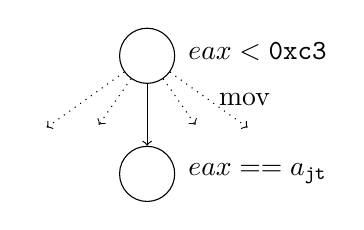
\begin{tikzpicture}
        \node[vertex]    (b)   at (3,-.5)    {};
        \node[draw=none] (120) at (1.6,-1.5) {};
        \node[draw=none] (121) at (2.3,-1.5) {};
        \node[vertex]    (122) at (3,-2)     {};
        \node[draw=none] (123) at (3.7,-1.5) {};
        \node[draw=none] (124) at (4.4,-1.5) {};

        \node[right] at (3.4,-.45) {$
          \reg{eax} < \mathtt{0xc3}
          $};

        \node[right] at (3.4,-2) {$
          \reg{eax} == a_\mathtt{jt}
          $};

        \draw [overlay,decorate,decoration={brace,amplitude=10pt,mirror},xshift=-4pt] (6,-1.75) -- (6,-.5) node [black,midway,xshift=1.4cm] {
          \begin{tabular}{l}
            up to $\mathtt{0xc3}$\\
            edges: one\\
            per read\\
            value
          \end{tabular}
        };

        \draw[dotted,->] (b)   to (120);
        \draw[dotted,->] (b)   to (121);
        \draw[->]        (b)   to (122);
        \draw[dotted,->] (b)   to (123);
        \path[dotted,->] (b)   edge node [right,xshift=0.2] {\inlineasm{mov}} (124);
      \end{tikzpicture}
    \end{example}
  \end{columns}
\end{frame}

\begin{frame}{Contribution \#4: Exceptional Interprocedural Control Flow Graphs}{Improvement on the state of the art}
  \centering
  \tikzstyle{backdraw}=[< draw] % Had to reenable bEnd1's ability to draw outgoing edges here as setting it on the edge itself didn't work.
  % Trying to use \only/\uncover/etc. with the graph paths directly doesn't work so need to mess with the styles
  \only<1>{
    \tikzstyle{unwind}=[draw=none]
    \tikzstyle{interproc}=[draw=none]
    \tikzstyle{bad}=[]
    \tikzstyle{good}=[]
    \tikzstyle{backdraw}=[]
  }
  \begin{tikzpicture}
    \graph[
    grow down=1.25cm,
    branch right=1.5cm,
    nodes={draw,ellipse,font=\ttfamily}
    ]{
      foo -> fEnd1/""[ret],
      foo -> "" -> {fEnd1, fEnd2/""[ret]}, % more compact this way
      foo'[landing] -> fEnd'/""[ret],

      bar -> {b1/"", bEnd1/""[ret,< draw=none]} -> {b2/"", bEnd2/""[ret]},
      b2 -> {bar[> bend left], bEnd2},
      b1 -> bEnd2, % necessary due to group/chain interactions
      bar'[landing] -> bEnd'/""[ret],

      {[grow down=1.25cm, branch right=1.5cm]
        {main[circle], catch[landing]} -> {
          callSite/""[diamond],
          ""[at=(0:-.5)],
          ""[ret, bad, at=(0:-1), < draw=none]
        } -> ""[ret,good],
      };

      callSite ->[interproc] foo;
      callSite ->[interproc] bar;

      fEnd1 ->[interproc] callSite;
      bEnd2 ->[interproc] callSite;

      fEnd2 ->[unwind] foo'; fEnd' ->[unwind] catch;
      bEnd1[backdraw] ->[unwind] bar'; bEnd' ->[unwind] catch;
    };
  \end{tikzpicture}
  \uncover<2->{
    \begin{description}[leftmargin=\widthof{Green triangle}]
      \item[Red dashes] normal interprocedural control flow
      \item[Blue dots] \alert{unwinding} edges
      \item[Green triangle] successful termination
      \item[Blue triangle] exceptional termination
    \end{description}
  }
\end{frame}

\subsection{Motivation}

\begin{frame}{Why static binary analysis?}
  \begin{outline}
    \1 Supports \alert{overapproximative} efforts
      \2 Requirement for \alert{soundness}
    \1 Allows analysis without source code
      \2 Legacy programs
      \2 Reverse engineering
        \3 Disassembly
        \3 Decompilation
      \2 Patching
      \2 Security analysis
    \2 Removal of compiler from the \gls{tcb}
  \end{outline}

  \todo{rotatebox with listing in the bottom right}
\end{frame}

\begin{frame}{Why \glsxtrlong{cfr}?}
  \begin{center}
    Required for static binary analysis: Existing disassemblers/decompilers often rely on external \gls{cfr} tools!
  \end{center}

  \todo{put a little figure to look nice}
\end{frame}

\begin{frame}{Why exceptional \gls{cfr}?}
  \begin{outline}
    \1 Common low(er)-level languages have structured exceptions, stack unwinding
      \2 \Gls{cpp} (\lstinline|throw|, \lstinline|try|, \lstinline|catch|) converted to standard \gls{abi} functions (\inlineasm{__cxa_throw}, etc.)
      \2 \Gls{c} with hooks to library functions
    \1 Can lead to \alert{unsoundness} if not modeled
  \end{outline}
\end{frame}

\begin{frame}{Novelty Restated}
  \todo{Figurify the outlines}
  \begin{columns}[t]
    \column{.4\textwidth}
    \begin{block}{Formally Verified Disassembly}
      \begin{outline}
        \1 Existing disassemblers \alert{unsound} % they make guesses or are not fully overapproximative
        \1 We are \alert{sound}!
      \end{outline}
    \end{block}

    \column{.5\textwidth}
    \begin{block}{\Glspl{eicfg}}
      \begin{outline}
        \1 Off-the-shelf \alert{disassemblers, decompilers} do not model exception unwinding
          \2 Ghidra % bib entries?
          \2 IDA Pro
          \2 Binary Ninja
        \1 We do!
      \end{outline}
    \end{block}
    \todo{Ghidra/etc. figures}
  \end{columns}
\end{frame}
